%% -*- coding: utf-8-unix -*-

\chapter{PoCターゲット設計}
\label{chap:poc-target-design}

PoCとしてユースケース実証実験をおこなう際に設定したPoCシナリオ(状況設定)、
PoC環境について解説する。

% TODO: ここにたどりつく前段階の検討のはなしをいれるか?
% アーキテクチャ検討_20160617.pptx
% https://drive.google.com/open?id=0B2eRR_JxYJA5RXdPTzVLU1M4RzQ

 \section{PoCの概要}
 \label{sec:poc-overview}

 % なんのために、どういったテストをおこなうのか。
 % そもそものPoCの考え方のまとめ・整理

 % 障害報告ストーリー – NetTester
 % \url{https://3.basecamp.com/3088280/buckets/867009/documents/151143879}
 % どういったサービス上のトラブルを検出したいとおもったのか? (ユースケース例)
 % 技術的にやりたいこと:  静的なテスト/動的なテスト

 \subsection{PoCの目的}
 \label{sec:poc-purpose}

\lopjc では network namespace によるテスト用ノード生成とOpenFlowスイッチ
による配置(パッチ)機能\footnote{\tabref{tab:test-functions}のNo.3,4に相
当する機能。}について基礎検証を実施した。本プロジェクトでは、その結果を
もとにNetTesterを実装し、実際のユースケースとしてどういったテストが自動
化可能か(\tabref{tab:test-functions}, No.5)を実証していく。テストのユー
スケースとして、静的なふるまい・動的なふるまいという、ふたつの観点でテス
トシナリオの実装を進める(\ref{sec:behavior-test}節)。

  \subsection{PoCターゲットユースケース検討}
  \label{sec:poc-usecase-discuss}

ネットワークテストのユースケースとして\tabref{tab:test-usecases}のような
事例について検討した。

\tabref{tab:test-usecases}の事例をもとに、汎用性があり、かつ「テストの自
動化」という観点で技術的に基礎となる機能を盛り込めるユースケースとして、
以下の2ケースを選択した。いずれも、テスト自動化の有効性を出しやすい条件を満たす
\begin{itemize}
 \item 頻繁に・繰り返しおこなう
 \item 複雑度が高く人によるレビュー等ではミスの発見が難しい
 \item 従来は人力にたよっており自動化が難しい
\end{itemize}
という観点で選択している。

\begin{itemize}
 \item FWのパケットフィルタポリシ運用
       \begin{itemize}
        \item 「静的なふるまい」の代表例として選択。
        \item FWポリシ管理(通信制御ポリシ管理)は、パターン数(ルール)が多
              く、順序の依存関係など複雑度の高い操作が求められるため。ま
              た日々の変更頻度が高く、運用管理コストの高い事例であるため。
        \item 特にアプリケーションレイヤ(L7)を検査するDPI機能を持つFWの
              テストは単純なL3/L4のツールでは自動化が難しい動作であるた
              め。
       \end{itemize}
 \item 冗長化構成FWのリンク障害試験
       \begin{itemize}
        \item 「動的なふるまい」の代表例として選択。(最も基本的な「動的
              なふるまい」の例としての物理トポロジ(物理リンク)操作。)
        \item 一般的に、FW(ハードウェアアプライアンス)はその機能や性能上
              の理由から製品ごとに固有のアーキテクチャを持つ\footnote{製
              品機能や性能を維持しつつ、FWを経由するセッションなどの情報
              (状態)をクラスタとして保持するため。}。そのため、特定のハー
              ドウェアやOSバージジョンで固有のバグが見つかることがある。
              こうした問題を事前に対処するためには、実際に本番環境で使用
              する実機(ハードウェア)を使用したテストが重要になる。
        \item クラスタ化されたFWのフェイルオーバー/フェイルバックはステー
              トフルな動作である。そのため、初期状態の設定、指定された手
              順を実行してネットワークの状態を遷移させていくオペレーショ
              ンが必要となる。また、状態遷移中の動作を複数並列してチェッ
              クしていく必要がある。いずれも従来は複数人で作業することで
              おこなっていたものだが、複数人による作業は全体の動作などが
              掴みにくいという問題があった。
       \end{itemize}
\end{itemize}

\begin{table}[hb]
 \centering
 \caption{テストユースケース案}
 \label{tab:test-usecases}
 \begin{tabularx}{\linewidth}{p{10em}|X}
  \hline
  ユースケース & 詳細(事例) \\
  \hline
  \hline
  ネットワーク移設時の通信不能 & ある拠点から他のDCへシステムを移設する際、現行システムのIPを継続するためにL2延伸をおこなっていた。しかし、上流側ネットワークでのルーティング経路トラブルにより通信ができなくなった。 \\ \hline
  FW通信誤許可 & 外部からhttpでアクセス不能なはずのシステムについて、実際には外部からのhttpでのアクセスが許可されていた。 \\ \hline
  システム拡張時の通信不安定 & システムの拡張時にL2ループが発生し通信が不安定になった。 \\ \hline
  FWの再起動による通信障害 & Active/Standby構成のFWでStandby側が再起動したときに、Active側が機能停止・冗長構成の情報交換ができず通信が停止した。\\ \hline
  通信遅延の発生、ネットワークのスローダウン & L3スイッチのリソース(メモリ・TCAM)枯渇による重大なネットワーク性能低下、通信遅延が発生した。 \\ \hline
  経路制御の設定ミスによるアクセス不能 & サーバリプレースによりシステム側のIPアドレスが変更となった際、一部機器でルーティング追加作業が漏れていたためにシステムへアクセス不能となった。 \\ \hline
  FW のリプレース & 古いFW機器(ハードウェア)を新しい世代の機器にリプレースする際、既存のルールを変換・インポートする操作に問題があり一部の通信が停止した。 \\ \hline
  FW フィルタ(ポリシ)のミスチェック & パケットフィルタが、フィルタ作成者の認識違いやミスなどで最終的に実現したいポリシになっていなかった。そのため、必要な通信の遮断・不要な通信の透過が発生してしまった。 \\
  \hline
 \end{tabularx}
\end{table}

  \subsection{PoC方針}

  % TODO みなおし -> https://drive.google.com/open?id=0B2eRR_JxYJA5Vm1Dd0dJRGdjWU0
ここまでで既にいくつか方針をあげているが、あらためてPoCの実施方針をまとめる。
\begin{itemize}
 \item 本PoCで実施すること
       \begin{itemize}
        \item テストシステムの機能・特定の自動化実装ではなく、「テストと
              して実行可能なユースケース」に注目する。
        \item ネットワークテストの基本的な考えかたとして「静的なふるまい
              のテスト」「動的なふるまいのテスト」の観点で実際のテストシ
              ナリオを実装する。
        \item 「ネットワークのふるまい」として、end-to-end通信の実現可否
              に着目する。ネットワークの設計・内部構造・使用している機材
              に関わらず、ネットワークとしてどういった通信が実現されるべ
              きか、という要求とそのテストに注目する。これは、ネットワー
              クの利用者あるいはネットワーク(サービス)提供者の視点から見
              た、ネットワークに対する期待\footnote{サービス提供者として、
              ネットワーク利用者にどういったサービスが提供できなければい
              けないか。}を確認することである。
       \end{itemize}
 \item 本PoCで実施しないこと
       \begin{itemize}
        \item 「できないこと」のテスト: 利用者あるいはサービス提供者の視
              点では、ネットワーク上「できてはいけないこと」の要求がある。
              例えば、隣接する他社顧客の環境と通信ができてはいけない、な
              ど。本PoCはまず利用者に対して最低限提供すべきサービス(「で
              きなければいけないこと」)についてのテストに焦点をあてる。
        \item 非機能要件のテスト(性能・拡張性・冗長性): 上記のとおり、本
              PoCではネットワークテスト(ユースケース)の実現可否、機能的
              な実現性に注目する。そのため、性能や拡張性などについては考
              慮せず、ユースケースを実現可能な最低限のシステム構成・実装
              をとることを方針としている。
       \end{itemize}
\end{itemize}

 \section{PoCターゲットの設定}

  \subsection{登場人物}
  \label{sec:poc-casting}

PoCにあたって\figref{fig:poc-situation}のように登場人物を設定した。
\begin{itemize}
 \item ヨーヨーダイン社\footnote{架空の企業名\cite{yoyodyne}}
       \begin{itemize}
        \item タジマックス通信工業社と共同でソフトウェア開発をおこなって
              いる。
        \item 社内ネットワークの新規構築をおこなうにあたり、ネットワーク
              の設計・構築についてもタジマックス通信工業社に発注すること
              になった。
       \end{itemize}
 \item タジマックス通信工業社\footnote{架空の企業名, プロジェクトメンバ
       の氏名から。}(以降 \tj )
       \begin{itemize}
        \item ソフトウェア開発および情報システム基盤の設計・構築などをお
              こなっている。
        \item ヨーヨーダイン社の社内ネットワーク設計構築を受注している。
       \end{itemize}
\end{itemize}

\begin{figure}[h]
 \centering
 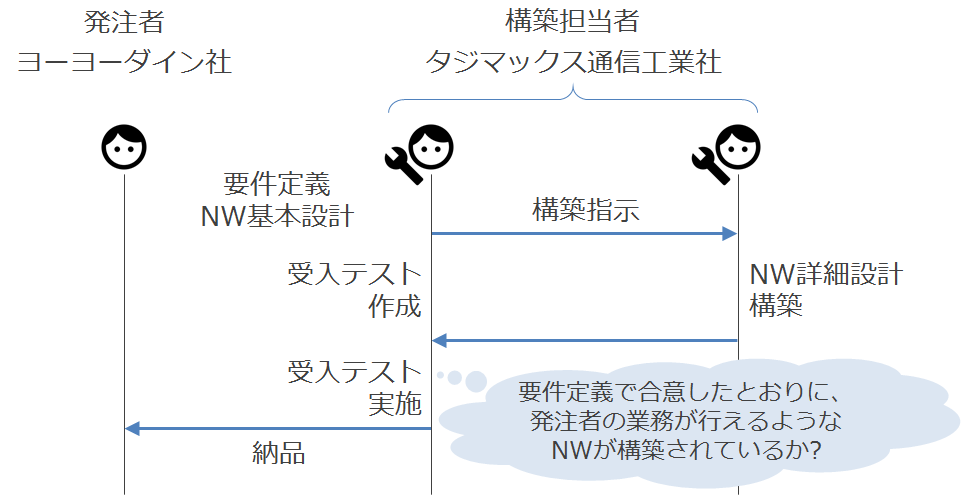
\includegraphics[scale=0.5]{img/poc-situation.png}
 \caption{PoC設定: 登場人物の位置付け}
 \label{fig:poc-situation}
\end{figure}

以降、ネットワークのテストシナリオについては、\tj 社員がテストをする視点
をとる。(\tj 社員がネットワークの設計・構築をおこない、\yo へ納入する前
に、\yo が業務をおこなう上で実現したいこと、\yo の要求すべてが問題なく実
現できているかどうかをテストする。)

\ref{chap:poc-scenario-dev}章で実際のテストシナリオ実装について解説する
が、PoCでは \tj 社員に相当するメンバとして次のように設定した。
\begin{itemize}
 \item ネットワークの要件定義・基本設計をおこなうネットワークエンジニア
 \item 決められたネットワーク要求に基づいてネットワークの構築をおこなう
       ネットワークエンジニア
 \item 決められたネットワーク要求に基づいてテストシナリオの実装・実行を
       おこなうソフトウェアエンジニア
\end{itemize}

今回、実際にPoCを進める際、次のようなプロジェクトメンバを設定している。
\begin{description}
 \item[ネットワークエンジニア担当(NW設計)] 顧客( \yo )要求をもとに、ネッ
            トワークの基本設計やテストシナリオの策定ができる。
 \item[ネットワークエンジニア担当(NW初期構築)] 通信要件やネットワーク基
            本設計をもとにFW/L3SW等の設定をおこなう。プログラミングやテ
            スト自動化についての知見をもたない。
 \item[ネットワークエンジニア担当(テスト実装・実行)] ネットワーク機器の
            設定や操作ができる。また、プログラミングの基本的な知識があり、
            小規模なスクリプトの実装ができる。テストシナリオ実行時に問題
            が発生した場合、テスト対象ネットワークおよびテストシナリオの
            どちらに原因があるかを切り分けることができる。
 \item[ソフトウェアエンジニア担当(テスト実装・実行)] ネットワーク
            (TCP/IP, Ethernet)の基本的な知識をち、ネットワーク要件に応じ
            て、どのようなテストを実行すべきか考えることができる。しかし、
            ネットワーク機器の設定などの知見をもたない。
 \item[ソフトウェアエンジニア担当(テスト設計・レビュー)] ソフトウェア開
            発と自動テストに関する経験をもち、テストシナリオ全体の方針策
            定、実装レビューを実施できる。ネットワークに関する基本的な知
            識はあるが、ネットワークの運用や操作についての知見はもたない。
\end{description}

  \subsection{サービス要件定義}

以下、PoC上の状況設定をおこなう。なお、PoCを複雑化させないため、原則
L1-L4の機能的な要件設定とし、(可用性を除く)非機能要件や主要な要件に付随
する業務上の要求\footnote{アクセスログ取得等セキュリティ観点の要求など。}は
設定しない。

    \paragraph{機能要件}
\yo および \tj が共同開発をおこなうための機能要件は次のようになる
\footnote{平成25年度のネットワークスペシャリスト試験の問題\cite{h25nwsp}
をもとに、架空の中小企業ネットワークとして設定している。}。
\begin{itemize}
 \item \yo は社内に開発環境を持つ。開発環境は社内からのみアクセス可能と
       する。
 \item \tj はインターネット経由で \yo 社内にアクセスし、開発環境を共用し
       て \yo との開発業務をおこなう。
       \begin{itemize}
        \item \tj からのアクセスはセキュアな通信方法をとること(通信を暗
              号化すること)
        \item \tj からのアクセスについて個人単位での認証・アクセスコント
              ロールができること。
       \end{itemize}
 \item \yo が社内外に提供するサービスは、インターネット環境に直接設置し
       ない。サービスの上流ネットワークで \yo によるL4(以上)のアクセス制
       御をおこなうこと。
 \item インターネット側から \yo 社内への通信を許可しない。(\yo がインター
       ネット側に提供するサービスを除く。)
\end{itemize}

    \paragraph{可用性}

ネットワークの可用性については次のように設定する。
\begin{itemize}
 \item インターネット回線の冗長化はおこなわない\footnote{PoC設定上の都合。
       障害試験ポイントとしてNW機器(FW)にのみ注目する。}。
 \item 社内では中核をなすNW機器の冗長化をおこなう。(機器メンテナンス作業
       や障害発生時の \tj 開発業務を継続するため。)
\end{itemize}

 \section{環境構成(Target Network)}
 % - L2/L3, Management network (VR/VRFとout-of-band設定)
 % - FWの冗長化設定:
 %        - active/passive, passiveはパケット転送しない
 %        - tcp session state を同期する
 %        - 状態監視するインタフェースの設定、自動復旧設定とする
 % - FWのフィルタ設定:
 %        - 原則L3/L4でのフィルタ
 %        - tcp state をみる
 %        - DNSについてはL7(DPI)でフィルタする

 % - IPアドレス表 \url{https://drive.google.com/open?id=1v0ecUjUql3cxVMP8gvLyq4T9PEIeUeyMT_-9YrR4l0A}

  \subsection{論理ネットワーク設計}
  \label{sec:logical-nw-design}

  \paragraph{利用者要件}
\tj は \yo とのネットワーク要件検討をもとに、
\figref{fig:poc-env-logical}・\tabref{tab:ip-list}のようなネットワークを
構築することとした。

\begin{itemize}
 \item \yo ネットワークは、外部(社外/インターネット)・DMZ・内部(社内)の
       セキュリティゾーンに分割する。
 \item 外部(external)ゾーン: インターネット接続用の固定IPセグメントをひとつ持ち、
       インターネット経由で外部へのサービスを提供できるようにする。
       \begin{itemize}
        \item グローバルIPアドレスは外部ゾーンのみで使用する。DMZおよび
              内部ゾーンではプライベートIPアドレスを使用する。社外(イン
              ターネット)との必要な通信についてのみ、外部ゾーン境界(FW)
              でNATをおこなう。
       \end{itemize}
 \item DMZゾーン: 外部に公開するサービスと内部に公開するサービスの中継を
       おこなう。
       \begin{itemize}
        \item SSL VPNサーバ: \tj との共同開発用に、インターネット経由で
              \tj からのリモートアクセスを受け付ける。\tj VPNクライアン
              トはVPN接続後、VPNサーバから割り当てられたDMZ内IPを使用し
              て内部ゾーンの開発環境にアクセスする。
        \item DNSサーバ: \yo 内部向けに提供する名前解決・サービス
       \end{itemize}
 \item 内部(internal)ゾーン: 社内のみ利用可能な開発系サーバおよび社員(開
       発用PC等)を設置する。
       \begin{itemize}
        \item 開発環境として、資産管理サーバ(Git)・内部テストサーバ
              (Telnet/Jenkins)を起く。
       \end{itemize}
 \item アクセスポリシとして、原則、内部--外部ゾーン間の通信はおこなえな
       いものとする。ただし、現状は内部ゾーン内機器からのNTPおよび
       HTTP/HTTPS通信に関しては直接外部ゾーンへ通すことを許可する
       \footnote{\tj は、\yo NW規模およびセキュリティポリシを検討した結
       果、現時点ではProxyサーバ導入をおこなわないものとした。}。
\end{itemize}

なお、\tj の設計・構築範囲は \yo ネットワークである。\tj ネットワークに
ついてはPoCの対象には含まれない。

\begin{figure}[h]
 \centering
 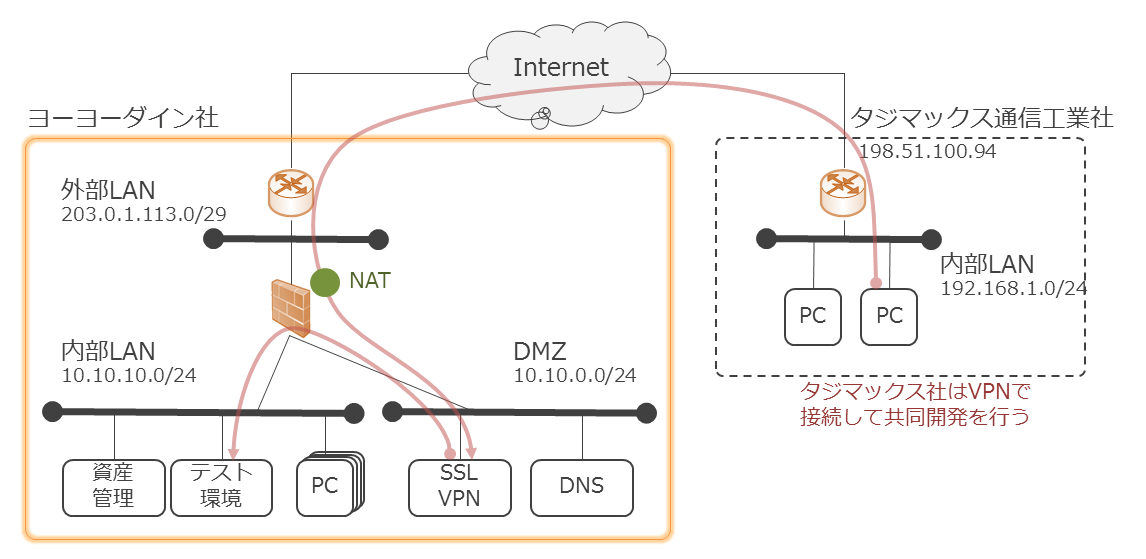
\includegraphics[scale=0.5]{img/poc-env-logical.png}
 \caption{PoC環境: 論理構成図}
 \label{fig:poc-env-logical}
\end{figure}

\begin{table}[h]
 \centering
 \caption{セグメント/IPアドレス一覧}
 \label{tab:ip-list}
 \begin{threeparttable}
  \begin{tabular}[t]{l|l|r|l}
   \hline
   Zone/Segment & IP Subnet & Local Host\tnote{1} & Host \\
   \hline
   \hline
   外部 & 203.0.113.0/29 & 0 & [Network] \\ \cline{3-4}
   & & 1 & Router \\ \cline{3-4}
   & & 2 & Firewall \\ \cline{3-4}
   & & 5 & SSLVPN ( \tj 社VPNアクセス) \\ \cline{3-4}
   & & 6 & NAPT (内部/DMZからInternetへのアクセス) \\ \cline{3-4}
   & & 7 & [Broadcast] \\ \hline
   DMZ & 10.10.0.0/24 & 0 & [Network] \\  \cline{3-4}
   & & 1 & Firewall (default gateway) \\ \cline{3-4}
   & & 10 & DNSサーバ \\ \cline{3-4}
   & & 11 & SSLVPNサーバ \\ \cline{3-4}
   & & 128-254 & SSLVPN Client IP Pool \\ \cline{3-4}
   & & 255 & [Broadcast] \\ \hline
   内部 & 10.10.10.0/24 & 0 & [Network] \\ \cline{3-4}
   & & 1 & 資産管理サーバ \\ \cline{3-4}
   & & 2 & テスト環境サーバ \\ \cline{3-4}
   & &  & 開発用PC \\ \cline{3-4}
   & & 254 & Firewall (default gateway) \\ \cline{3-4}
   & & 255 & [Broadcast] \\
   \hline
  \end{tabular}
  \begin{tablenotes}
   \footnotesize
   \item[1] 第4オクテット
  \end{tablenotes}
 \end{threeparttable}
\end{table}

    \paragraph{管理者要件}
ネットワークや各種サービスを運用・管理するための要求を以下のように設定する。
\begin{itemize}
 \item サーバ管理アクセス: 内部/DMZゾーンにおかれるサーバについては、\yo
       開発者が管理者を兼任しており、内部ゾーンから直接リモートアクセス
       することで運用・管理作業をおこなう。(in-band management)
 \item ネットワーク管理アクセス: ネットワーク機器の運用管理については、
       構築した \tj 社員をおくことを想定し、\yo ネットワークとは分離した
       設計とする。詳細については\ref{sec:mgmt-and-tester-nw}節参照。
\end{itemize}

  \subsection{通信要件}
  \label{sec:network-requirements}

利用者要件および管理者要件をふまえて、ネットワークで提供する通信要件は
\tabref{tab:poc-requires-yo-int}・\tabref{tab:poc-requires-yo-dmz}・
\tabref{tab:poc-requires-etc} のようになる。

\begin{landscape}
 \begin{table}[h]
  \centering
  \caption{PoC 通信要件(ヨーヨーダイン社内部セグメント起点)}
  % No.1-12
  \label{tab:poc-requires-yo-int}
  \begin{threeparttable}
   \begin{tabularx}{\linewidth}{c|X|X|X|X|X|X|X}
\hline
No. & ポリシ & アプリケーション & \multicolumn{2}{|l|}{Source IP} & \multicolumn{2}{l|}{Destination IP} & Destination Port \\
\hline
\hline
1 & PC→開発環境 & Git & PC & 10.10.10.0/24 & 資産管理サーバ & 10.10.10.1 & tcp/11000 \\ \hline
2 & PC→開発環境 & Telnet & PC & 10.10.10.0/24 & テスト環境サーバ & 10.10.10.2 & tcp/23 \\ \hline
3 & PC→開発環境 & Jenkins & PC & 10.10.10.0/24 & テスト環境サーバ & 10.10.10.2 & tcp/13000 \\ \hline
4 & PC→開発環境 & サーバ管理: ssh & PC & 10.10.10.0/24 & 資産管理サーバ & 10.10.10.1 & tcp/22,80,443 \\ \hline
5 & PC→開発環境 & サーバ管理: ssh & PC & 10.10.10.0/24 & テスト環境サーバ & 10.10.10.2 & tcp/22,80,443 \\ \hline
6 & PC→DNSサーバ & DNS Query & PC & 10.10.10.0/24 & DNSサーバ & 10.10.0.10 & tcp,udp/53 \\ \hline
7 & PC→Internet & Web browsing & PC & 10.10.10.0/24 & Internet & ANY & tcp 80,443 \\ \hline
8 & PC→Internet & NTP Query & PC & 10.10.10.0/24 & Internet & ANY & udp/123 \\ \hline
9 & PC→DNSサーバ & 応答確認: ping/traceroute & PC & 10.10.10.0/24 & DMZ & 10.10.0/24 & icmp \\ \hline
10 & PC→Internet & 応答確認: ping/traceroute & PC & 10.10.10.0/24 & Internet & ANY & icmp \\ \hline
11 & PC→DNSサーバ & サーバ管理: ssh & PC & 10.10.10.0/24 & DNSサーバ & 10.10.0.10 & tcp/22 \\ \hline
12 & PC→SSLVPNサーバ & サーバ管理: ssh, webui & PC & 10.10.10.0/24 & SSLVPNサーバ & 10.10.0.11 & tcp/22,80,443 \\ \hline
   \end{tabularx}
   \begin{tablenotes}
    \footnotesize
    \item ヨ社: ヨーヨーダイン社
    \item タ社: タジマックス通信工業社
   \end{tablenotes}
  \end{threeparttable}
 \end{table}
\end{landscape}

% AP1 : Git
% AP2 : Telnet
% AP3 : Jenkins

\begin{landscape}
 \begin{table}[h]
  \centering
  \caption{PoC 通信要件(ヨーヨーダイン社DMZセグメント起点)}
  % No.13-24
  \label{tab:poc-requires-yo-dmz}
  \begin{threeparttable}
   \begin{tabularx}{\linewidth}{c|X|X|X|X|X|X|X}
\hline
No. & ポリシ & アプリケーション & \multicolumn{2}{|l|}{Source IP} & \multicolumn{2}{l|}{Destination IP} & Destination Port \\
\hline
\hline
13 & DMZ→Internet & package update (web) & DMZ内サーバ & 10.10.0.0/25 & Internet & ANY & tcp/80,443 \\ \hline
14 & DNSサーバ→DNS Query & 上位DNSへのクエリ & DNSサーバ & 10.10.0.10 & Internet & ANY & tcp,udp/53 \\ \hline
15 & DMZ→DNSサーバ & DNS Query & DMZ内サーバ & 10.10.0.0/25 & DNSサーバ & 10.10.0.10 & tcp,udp/53 \\ \hline
16 & DMZ→NTP & NTP Query & DMZ内サーバ & 10.10.0.0/25 & Internet & ANY & udp/123 \\ \hline
17 & PC→DNSサーバ & ヨ社内部 & PC & 10.10.10.0/24 & DNSサーバ & 10.10.0.10 & tcp,udp/53 \\ \hline
18 & PC→DMZ & サーバ管理: ssh & PC & 10.10.10.0/24 & DMZ内サーバ & 10.10.0.0/25 & tcp/22,80,443 \\ \hline
19 & VPNPOOL→開発環境 & Git & DMZ VPN Pool & 10.10.0.128/25 & 資産管理サーバ & 10.10.10.1 & tcp/11000 \\ \hline
20 & VPNPOOL→開発環境 & Telnet & DMZ VPN Pool & 10.10.0.128/25 & テスト環境サーバ & 10.10.10.2 & tcp/23 \\ \hline
21 & VPNPOOL→開発環境 & Jenkins & DMZ VPN Pool & 10.10.0.128/25 & テスト環境サーバ & 10.10.10.2 & tcp/13000 \\ \hline
22 & DMZ→Internet & 応答確認: ping/traceroute & DMZ内サーバ & 10.10.0.0/25 & Internet & ANY & icmp \\ \hline
23 & DMZ→ヨ社内部 & 応答確認: ping/traceroute & ヨ社内部 & 10.10.10.0/24 & DMZ内サーバ & 10.10.0.0/25 & icmp \\ \hline
24 & ヨ社内部→DMZ & 応答確認: ping/traceroute & DMZ内サーバ & 10.10.0.0/25 & ヨ社内部 & 10.10.10.0/24 & icmp \\ \hline
   \end{tabularx}
   \begin{tablenotes}
    \footnotesize
    \item ヨ社: ヨーヨーダイン社
    \item タ社: タジマックス通信工業社
   \end{tablenotes}
  \end{threeparttable}
 \end{table}
\end{landscape}

\begin{landscape}
 \begin{table}[h]
  \centering
  \caption{PoC 通信要件(Internet/タジマックス社セグメント起点)}
  % No.25-28(Internet), No.29-30(タ社)
  \label{tab:poc-requires-etc}
  \begin{threeparttable}
   \begin{tabularx}{\linewidth}{c|X|X|X|X|X|X|X}
\hline
No. & ポリシ & アプリケーション & \multicolumn{2}{|l|}{Source IP} & \multicolumn{2}{l|}{Destination IP} & Destination Port \\
\hline
\hline
26 & Internet→外部 & 応答確認: ping/traceroute & Internet & ANY & Router & 203.0.113.1 & icmp \\ \hline
27 & Internet→外部 & 応答確認: ping/traceroute & Internet & ANY & Firewall & 203.0.113.2 & icmp \\ \hline
28 & 外部→Internet & 応答確認: ping/traceroute & ヨ社外部 & 203.0.113.0/29 & Internet & ANY & icmp \\ \hline
29 & PC→ヨ社VPN & SSLVPN & タ社(Global) & 198.51.100.94 & SSLVPNサーバ & 203.0.113.5 & tcp/80,443 \\ \hline
30 & PC→ヨ社VPN & 応答確認: ping/traceroute & タ社(Global) & 198.51.100.94 & SSLVPNサーバ & 203.0.113.5 & icmp \\ \hline
   \end{tabularx}
   \begin{tablenotes}
    \footnotesize
    \item ヨ社: ヨーヨーダイン社
    \item タ社: タジマックス通信工業社
   \end{tablenotes}
  \end{threeparttable}
 \end{table}
\end{landscape}

  \subsection{物理ネットワーク設計}
  \label{sec:physical_nw_design}

    \paragraph{物理設計の基本的な考えかた}
論理ネットワーク設計(\ref{sec:logical-nw-design}節)をもとに、物理ネット
ワーク設計を\figref{fig:poc-env-physical}のようにした。使用した機器の詳
細については\tabref{tbl:device-list}参照。
\begin{itemize}
 \item セキュリティゾーンおよびゾーン間通信ポリシはFirewallによっておこ
       なう。
       \begin{itemize}
        \item 外部: WAN/Untrust Zone
        \item DMZ: DMZ Zone
        \item 内部: LAN/Trust Zone
       \end{itemize}
 \item 外部ゾーンはFW上流側L3SWで収容する。L3SWはinternet境界(キャリア回
       線終端)である。
 \item 内部ゾーンおよびDMZはL2SW1/L2SW2で収容する。物理リンクは共有し、
       VLANによって論理的に分離する。
\end{itemize}

管理系ネットワークについてはサービス系ネットワークと分離する
(\ref{sec:mgmt-and-tester-nw}節)。

    \paragraph{冗長性}

社内ネットワーク冗長化の要求からFirewallを冗長化する。
\begin{itemize}
 \item FirewallはActive/Passive方式とする。障害が発生していない場合はFW1
       が通常Activeとなり、トラフィックの転送をおこなうものとする。
 \item Active側FW(FW1)のもつすべてのリンクについて、いずれかひとつでもリ
       ンクダウンが発生した場合に自動的に処理をPassive側(FW2)へ切り替え
       る。
 \item 切替のトリガとなったリンクダウンが復旧し、FW1の全リンクが正常になっ
       た場合は、トラフィック処理をFW1へ切り戻す。
 \item ステートフルフェイルオーバー: FW1/FW2は常に処理しているセッション
       の情報を同期し、切替・切り戻しが発生した際でも処理中のトラフィッ
       ク(セッション)を維持する。
\end{itemize}

    % \paragraph{パケットフィルタ}
    % DNSのテスト作る – NetTester
    % https://3.basecamp.com/3088280/buckets/867009/todos/301325453
    % SSGでDNS DPIするみたいな記述はみあたらない。
    % どう書くか...

% Firewall では基本的にL3/L4のパケットフィルタをおこなう(ステートフルイン
% スペクション可能)。

\begin{figure}[h]
 \centering
 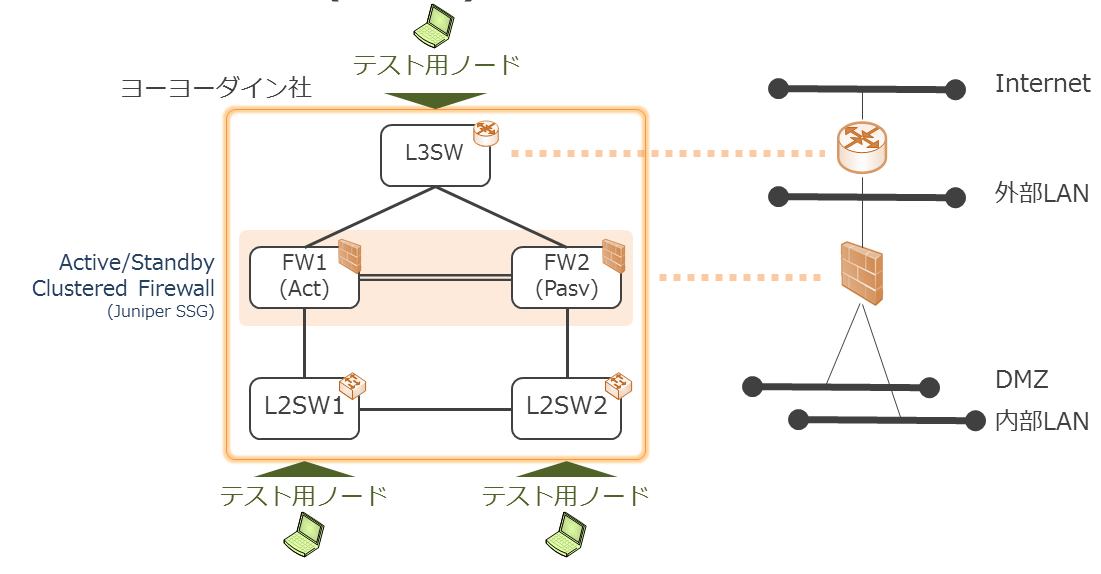
\includegraphics[scale=0.55]{img/poc-env-physical.png}
 \caption{PoC環境: 物理構成図(概要)}
 \label{fig:poc-env-physical}
\end{figure}

\begin{table}[h]
 \centering
 \caption{機器一覧}
 \label{tbl:device-list}
 \begin{tabular}[t]{l|l|l|l}
  \hline
  Host & Vendor & Device & Version \\
  \hline
  \hline
  FW1/2 & Juniper & SSG20 & ScreenOS 6.3.0r22.0 \\ \hline
  L3SW, L2SW1/2 & Cisco & Catalyst3750G-24TS & IOS 12.2(50)SE5 (ipservicesk9) \\ \hline
 \end{tabular}
\end{table}

% SSG, 当初使用していたのは 6.3.0r5.0

 \section{環境構成(管理系およびテストシステム)}
 \label{sec:mgmt-and-tester-nw}
 % - Tester Set について
 % - 構成図 \url{https://drive.google.com/open?id=0B2eRR_JxYJA5Nm1VbzBnR1FQMUk}
 % - Syslogについて

管理者要件(\ref{sec:logical-nw-design}節)のとおり、ネットワーク管理につ
いては \yo サービスネットワークと分離した構成をとる。
\figref{fig:poc-env-physical}のネットワーク機器(FW, L2/L3スイッチ)管理ア
クセスについては、次のように out-of-band な管理ネットワークを構成する
(\figref{fig:poc-env-physical-detail})。
\begin{itemize}
 \item Firewall: 管理用VRを設定し、管理用VRへ接続するインタフェースおよ
       びVLANをサービス用のものと分離する。
 \item L2/L3スイッチ: 管理用VRFを設定し、管理用VRFへ接続するインタフェー
       スおよびVLANをサービス用のものと分離する。
\end{itemize}

    \paragraph{Tester set}
\figref{fig:model-nettester}のように、NetTester server と対応する物理
OpenFlowスイッチのペアを、本プロジェクトでは「Tester Set」と呼ぶ。
NetTesterによるテスト作業は tester set の範囲内でおこなわれる。

PoCにあたって、検証環境(\figref{fig:poc-env-physical-detail})内ではふた
つのtester setを構築した。これは次の理由によるものである。
\begin{itemize}
 \item テストシナリオ実装のうち、実装・テスト実行\footnote{テストシナリ
       オの動作テスト}・デバッグ作業について、可能な範囲で並行して作業で
       きるようにするため。
 \item NetTesterのデバッグ、バグ再現調査などトラブルシュート対応における
       原因切りわけ手段として。機器故障や環境依存のある問題を切りわけ、
       作業中断リスクを回避するため。
\end{itemize}

    \paragraph{Tester setによるテスト実装作業の制限}
テスト実行は原則としてひとつのtester setで実行されることを想定する
\footnote{ひとつのサーバ(OS)上で複数のNetTesterは実行できない。複数の
NetTester serverをまたいで排他制御をおこなう制御はNetTesterではなく外部
オーケストレータなどで実行する必要がある
(\ref{sec:testscenario-excl-ctrl}節)。}。並行作業や同時実行については以
下のような条件について考慮する必要がある。
\begin{description}
 \item[テストシナリオ中で使用するテスト用ノード等のパラメタ重複] 例えば、
            同一IPのテスト用ノードを生成するテストシナリオを、ひとつのテ
            スト対象ネットワーク内で同時に実行するような場合。(デバッグ
            や調査などで同一シナリオを異なるtester setで同時に実行すると
            いったケース)。
 \item[テスト実行中(実行前後)のテスト対象ネットワーク状態遷移] 例えば、
            リンク障害試験(「動的なふるまいのテスト」)では、操作対象とな
            る物理リンクが1箇所となる。よって、その物理リンクを制御可能
            なtester setはひとつだけに限られる。
            \begin{itemize}
             \item 同様に、「静的なふるまいのテスト」はテスト実行中にト
                   ポロジなどネットワーク自体の構造が変化する想定をおい
                   ていない。そのため、「動的なふるまいのテスト」と同時
                   に実行することはできない。
            \end{itemize}
\end{description}

\figref{fig:poc-env-physical-detail}ではtester set 1を「動的なふるまいの
テスト」用に使用するように設計している。テスト対象が物理ネットワークであ
り、ひとつのインスタンスからのみ操作可能なリソースがある点に注意が必要で
ある\footnote{NetTesterに外部から操作可能なAPIを実装して連携させるといっ
た応用も考えられるが、こうした応用は本プロジェクトの目標範囲外となる。}

    \paragraph{物理構成図補足}
\figref{fig:poc-env-physical-detail}にあるSSG5はFW(FW1/2)の設定や動作確
認用に使用したものである(OSはFW1/2と同様: \tabref{tbl:device-list})。
NetTester開発やテストシナリオ実装にあたって、FWの設定や挙動をテストシナ
リオ上から確認し、問題点の切りわけをおこなうために利用した。

\begin{landscape}
 \begin{figure}[h]
  \centering
  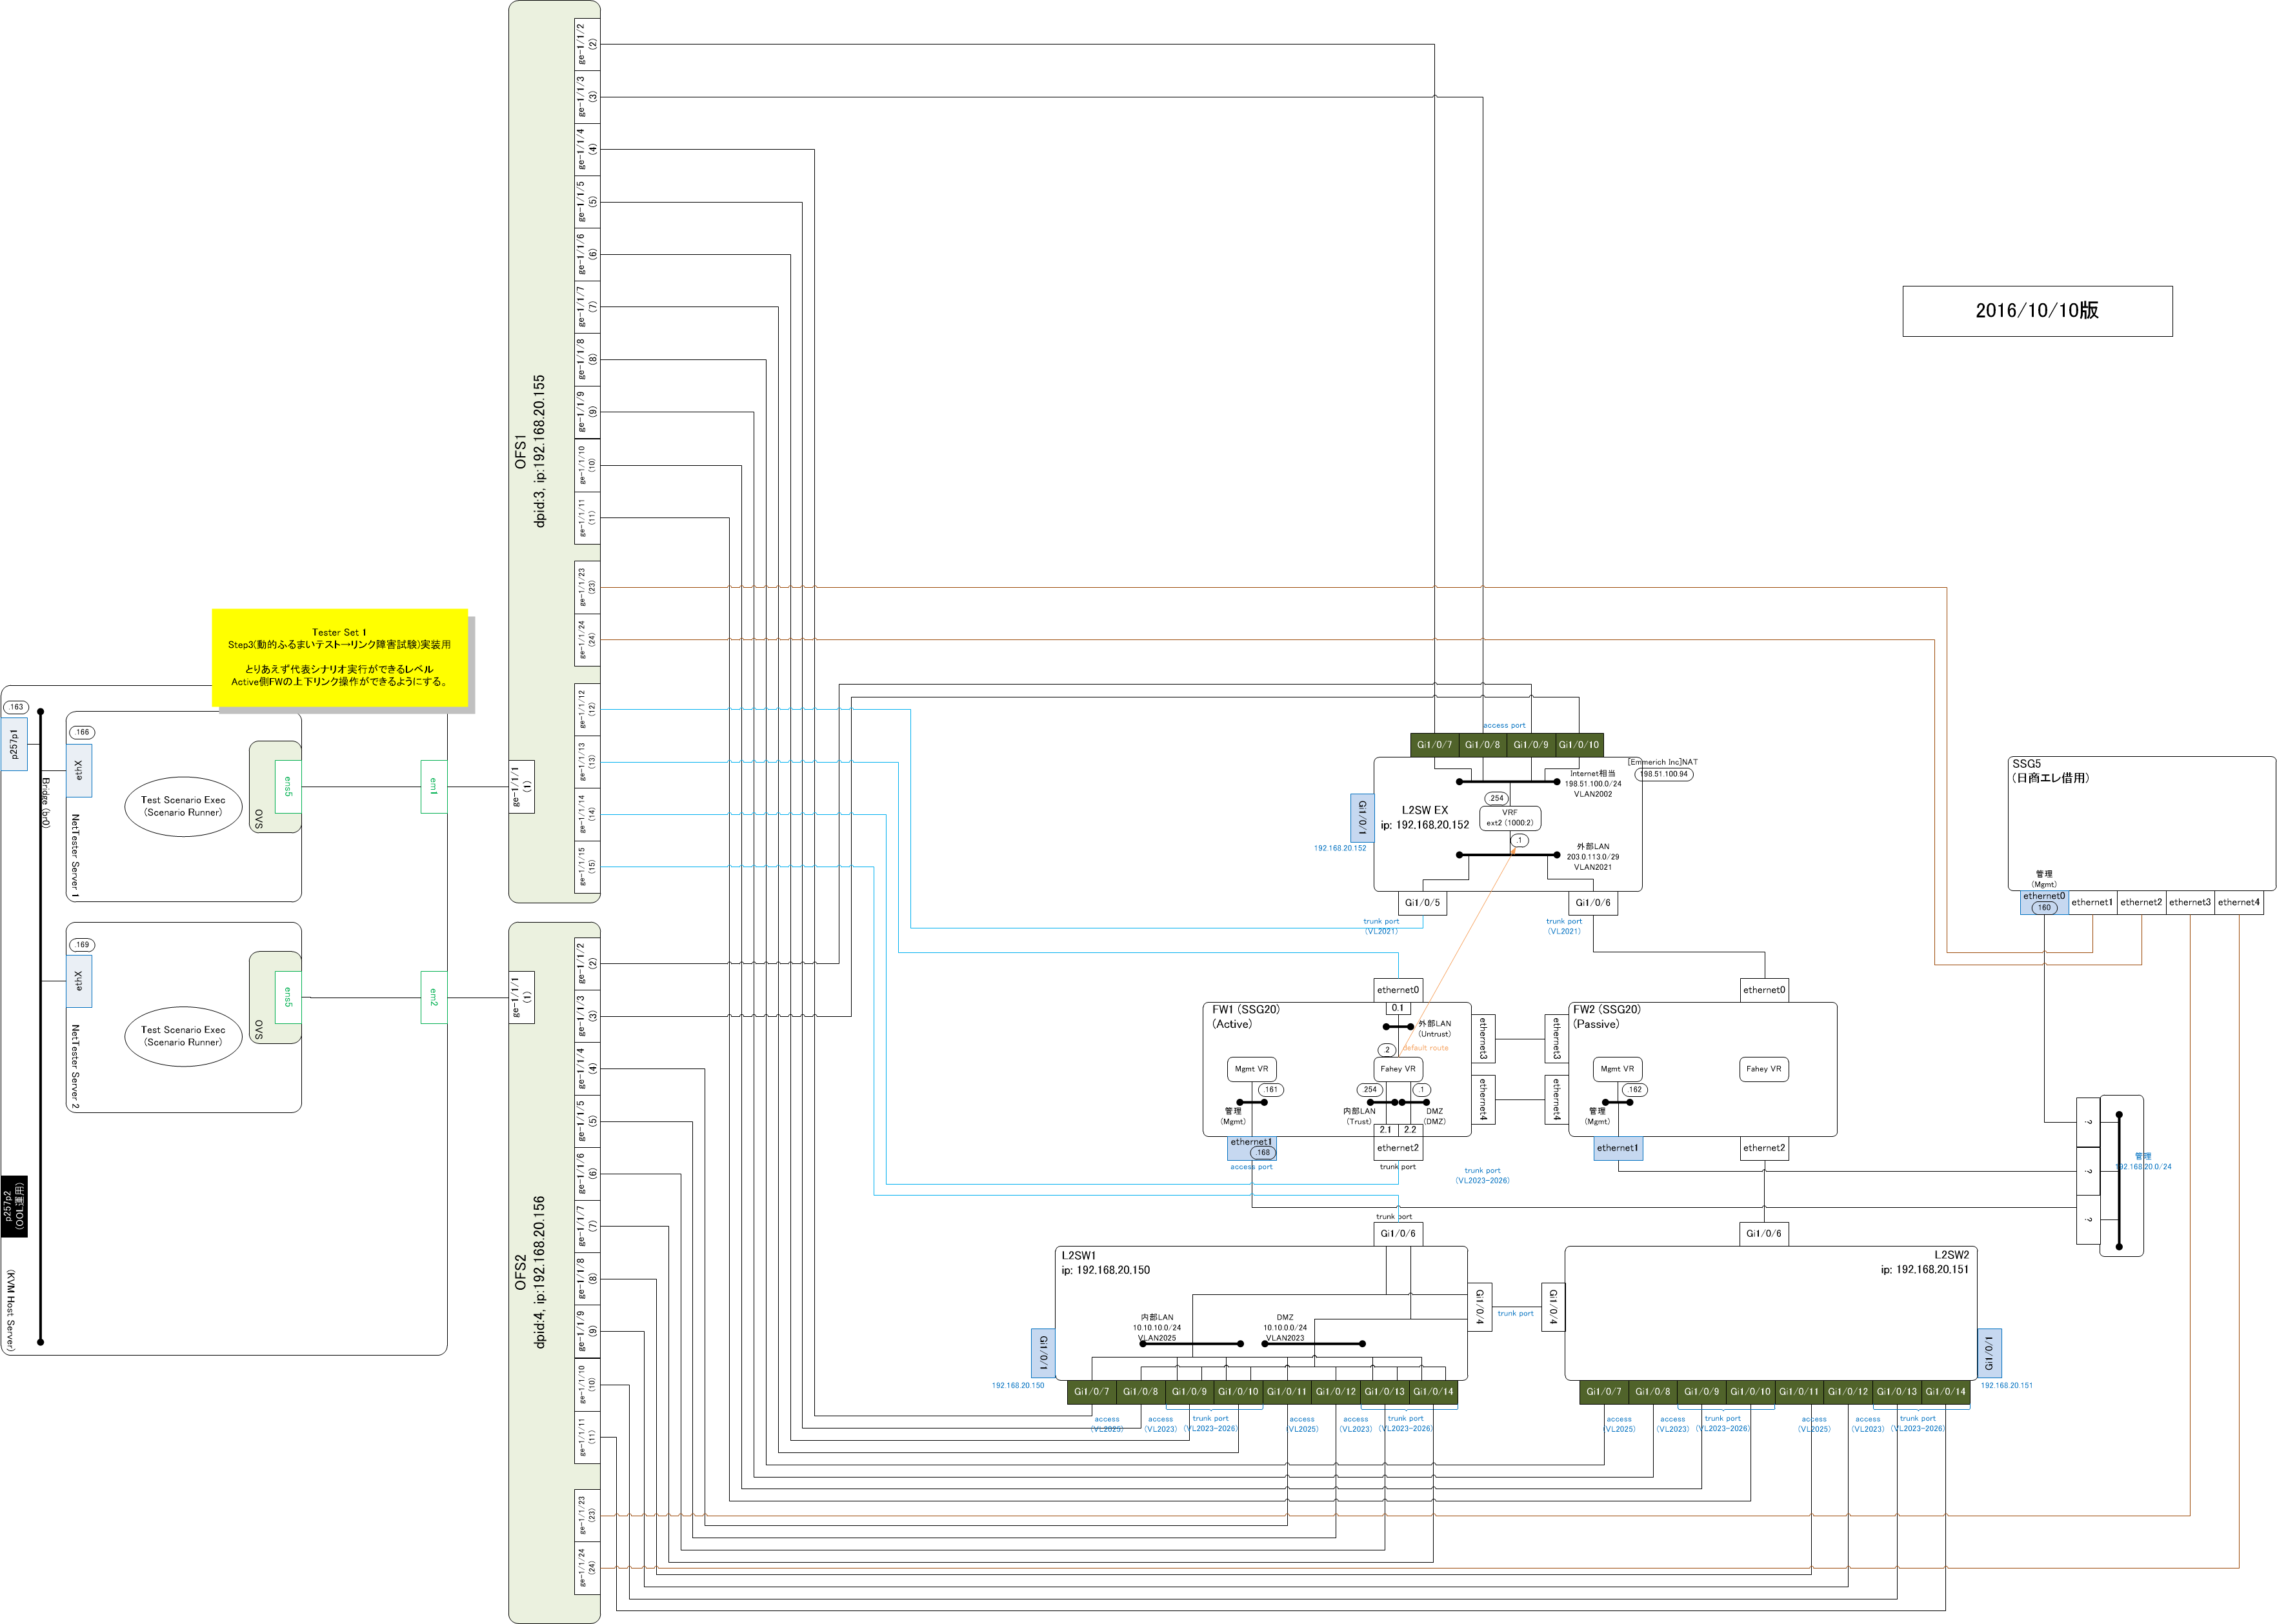
\includegraphics[scale=0.225]{img/poc-env-physical-detail.png}
  \caption{PoC環境: 物理構成図(詳細)}
  \label{fig:poc-env-physical-detail}
 \end{figure}
\end{landscape}


%%% Local Variables:
%%% mode: yatex
%%% TeX-master: "main.tex"
%%% End:
